Une large partie de la théorie des données fonctionnelles suppose que l'on observe des courbes $X_i : \Omega \rightarrow \mathcal C^0(I, \mathds R)$ \textbf{indépendantes} et identiquement distribuées. Cependant une partie non négligeable des données que l'on observe ont des dépendances avec les valeurs passées. Par exemple, il est raisonnable de penser que la consommation électrique d'un foyer au cours d'une année croît avec l'ajout successif de nouveau appareils électroniques. L'hypothèse d'indépendance entre les données n'est donc plus pertinente pour les données que l'on traite et il devient important de considérer des processus autorégressifs adaptés aux données fonctionnelles.
Si dans le cadre des données de $\mathds R$ cette relation de \emph{dépendance linéaire} avec le passé pouvait s'écrire sous la forme suivante
$X_n = \sum\limits_{k=1}^{n-1} \varphi_k \, X_k + \xi_n$ où $\varphi_k \in \grandR$
et
$\xi_n \begin{cases} \in \operatorname{VA}(\grandR) \\ \indep \sigma\left( X_i \right)_{1\,: \, n-1}\end{cases}$,
dans le cadre fonctionnel on capture la même idée en considérant
$X_n = \sum\limits_{k=1}^{n-1} \phi_k \left( X_k \right) + \xi_n$ où $\phi_k$
est un \emph{opérateur linéaire} de $\mathds L^2(I, \mathds R)$,
le plus souvent intégral.

\chk{
	Il s'agit d'une généralisation naturelle de la relation dans le cadre réel, puisqu'on peut démontrer que sur l'espace des nombres réels l'ensemble des fonctions linéaires $\phi : \grandR \rightarrow \grandR$ sont de la forme $x \mapsto ax$ avec $a \in \grandR$. La relation sur $\grandR$ que l'on a vue juste avant peut alors se ré-écrire de façon similaire à la version fonctionnelle.
}

On considère lors de ce stage des séries temporelles de données fonctionnelles car les données que l'on manipule ( en l'occurence les données de courbe de charge des parcs éoliens ) semblent être naturellement corrélées dans le temps.


\question{Pourquoi se soucier en particulier des séries temporelles fonctionnelles lorsque l'on souhaite incorporer la régularité du processus dont est issu nos données dans l'estimation des quantités qui nous intéressent ?}

Rappelons-nous que les données fonctionnelles sont la clé pour déterminer la régularité, et que cela est en réalité permis par le théorème de \nameref{rem:kolmo_continuite} (que nous n'avons pas énoncé en détails, mais mentionné dans la section \ref{sec:informel}). Malheureusement, dans le monde réel où vit le praticien, nous n'avons pas accès à l'espérance de la loi dont sont issues nos données. Il nous faut donc estimer cette espérance, et c'est là que les séries temporelles fonctionnelles entrent en jeu. Puisque l'estimateur usuel de l'espérance est la moyenne empirique, qui nous est fourni par la loi des grands nombres, cela devient très problématiques lorsque l'on dispose de données corrélées.
% TODO ✏️ mieux formuler - dépendance faible -> LGN faible -> estim esperance
Ce que nous allons voir, c'est que l'on peut tout de même utiliser l'estimateur usuel de l'espérance, et que l'on obtiendra des estimateurs des paramètres de régularité convergents ponctuellement vers ceux du processus dont sont issues nos données. Ce résultat est dérivé en utilisant une forme particulière de dépendance que le lecteur pourra étudier plus en détail en annexe \ref{annexe:regularite-locale}.

\begin{figure}[H]
	\centering
	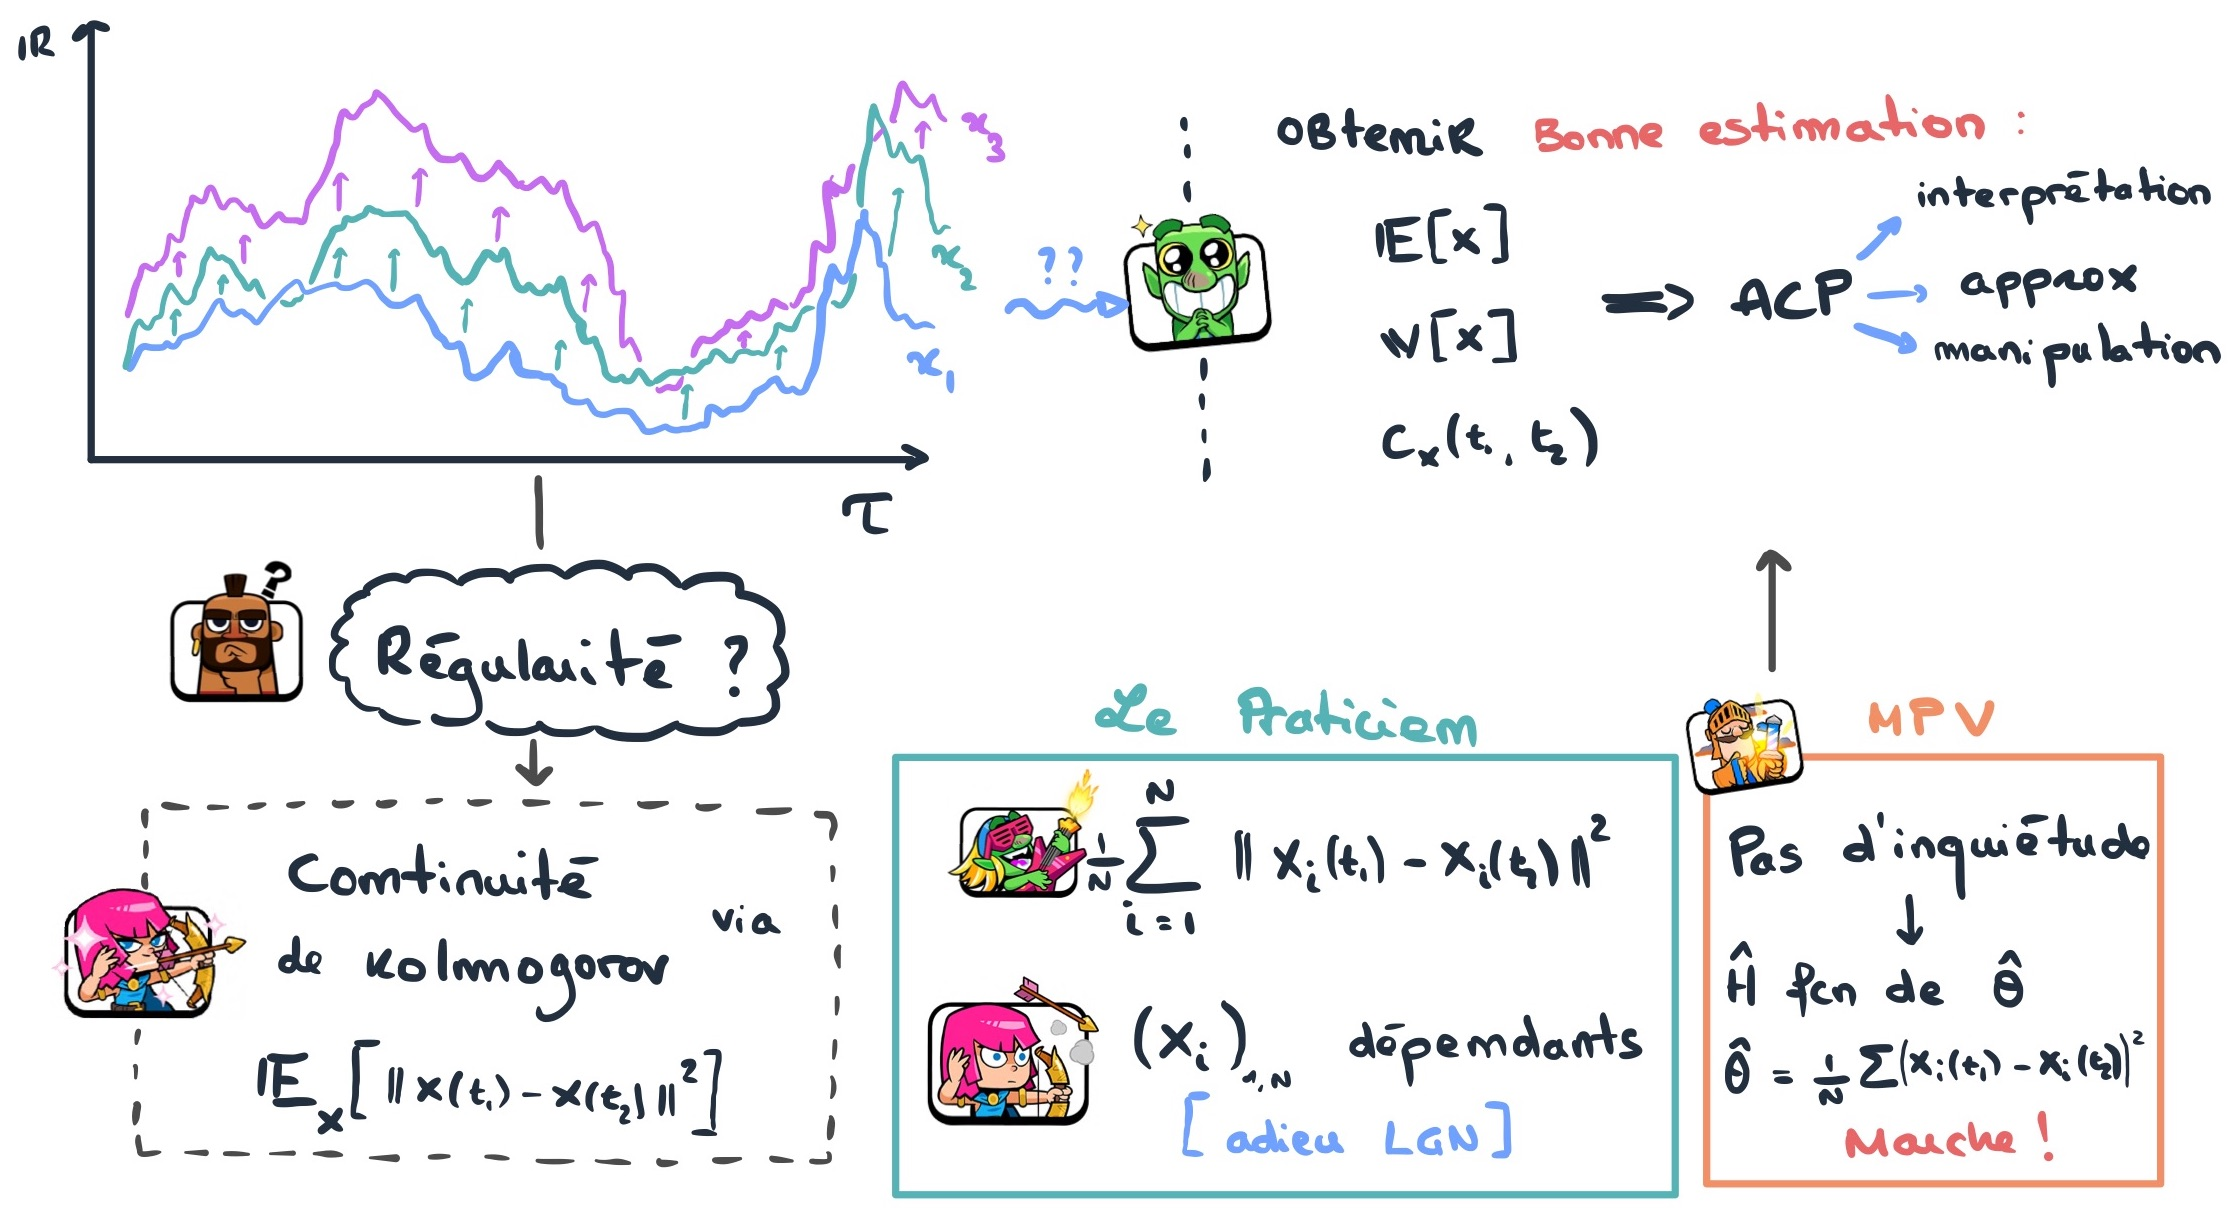
\includegraphics[width=\textwidth]{Images/sketches/schema_ts_estim_reg.jpg}
	\caption{Schéma grossièrement récapitulatif : Estimation de la régularité pour une série temporelle fonctionnelle}
	\label{fig:recap_estim_reg_fts}
\end{figure}


\warn{Il faut faire attention lorsque l'on manipule ou interprète des séries temporelles fonctionnelles. (comme par exemple tout résultat utilisant la loi de $\sum\limits_n X_n$, ... )}

Une série temporelle discrète est le fait que l'observation suivante dépend linéairement de l'observation précédente, dans le cadre fonctionnel \emph{l'observation est une fonction}. La dépendance se fait sur l'indice de la fonction, et non pas sur l'argument de la fonction interprété dans notre caps comme étant le temps.

\bigskip

Dans le cadre éolien c'est d'autant plus trompeur de parler de temps car on observe des courbes de charge sur une année : à la fois l'indice de la fonction et l'argument de la fonction ont des interprétations temporelles.

\smallskip

\noindent\fbox{%
    \parbox{\textwidth}
    {%
        dans l'expression \og$X_n(t)$\fg, la série temporelle (discrète) concerne bien l'indice $n$ et non pas l'argument $t$.
    }
}

\bigskip

\noindent La question devient alors :
\question{Lorsque l'on a une dépendance dans les observations fonctionnelle $\left\{ X_1 \dots X_n \right\}$, possède-t-on une dépendance dans les observations ponctuelles à $t$ fixé $\left\{ X_1(t) \dots X_n(t) \right\}$ ? Cette dépendance est-elle la même ?}

\noindent Et la réponse, c'est qu'\textbf{on ne sait pas}. En tout cas, dans le cadre général. Il y a en effet plusieurs façon de définir ce qu'on appelle par \og dépendance temporelle \fg. Toutes les définitions de dépendance ne mènent pas à cette conclusion, mais celle adoptée par (MPV) l'est, étant plus faible. De manière générale, lorsque l'on traîte des données avec de la dépendance, il convient d'être extrêmement précautionneux avec les théorèmes et \og faits \fg que l'on invoque. Toujours bien vérifier les hypothèses.


Il y a dans un premier temps ce qu'on appelle la dépendance \og forte \fg, comme la dépendance dite de \og $\alpha$-mixing \fg comme définie dans ~\cite{estimation-dependent-strong-mixing} :


\begin{definition*}[$\alpha-$mixing]

    une suite $X = \suite X i$ de variables aléatoire est dite $\alpha$-mixing si pour tout $n \in \mathds N$


    $$
        \alpha(n) \tend n \infty 0
    $$

    avec : $\alpha(n) = \sup\limits_k \bigl\{ \lvert \proba{A \cap B} - \proba{A}\proba{B} \rvert \quad | \quad A \in \sigma( X_{1:k} ), \, B \in \sigma(X_{k+n : \infty}) \bigr\}$

    en d'autres termes, la \og dépendance \fg \colorize[flatuicolors_blue_devil]{$(\lvert\, \proba{A \cap B} - \proba{A}\proba{B} \,\rvert)$} entre les variables aléatoires $X_k$ et $X_{k+n}$ tend vers 0 lorsque $n$ tend vers l'infini.
\end{definition*}

Ce point de vue est \og fort \fg dans le sens où l'on manipule directement les tribus, et que l'on regarde leur degré d'indépendance via la mesure de probabilité. Il ne s'agit pas de l'approche considérée par MPV qui est plus faible, en se reposant non pas sur l'indépendance des tribus engendrées par la série temporelle mais en exploitant la qualité d'approximation de la série temporelle que l'on étudie par un autre processus, indépendant de la série temporelle étudiée à partir d'un certain rang. La définition de dépendance temporelle est alors dite \og faible \fg. Le point de vue faible offre un comportement plus sympathique pour l'aspect \emph{local} dans l'estimation de la régularité : qui est le coeur de l'approche de MPV.


\bigskip

Les processus qui nous intéressent et ceux auxquels on va se limiter dans un premier temps sont les processus causaux. Comme dans le cas réel, on peut étudier les séries temporelles en posant l'opérateur :

$$B : x_n \mapsto x_{n-1}$$

et la relation de dépendance encodée par :

$$X_{n-1} = \phi(X_n) + \xi_n \qquad \phi \; \textsf{linéaire}$$

Si le processus est inversible, on peut écrire $X_n$ comme le développement en série entière suivant :

\begin{align*}
    X_n                                  & =                                         & \phi \circ B(X_n) + \xi_n                                                                       \\
    \left[I - (\phi \circ B)\right](X_n) & \underset{\textsf{}} =                    & \xi_n
    \\
    X_n                                  & \underset{\Vert \phi \circ B \Vert < 1} = & \inverse{[\phi \circ B]} (\xi_n)
    \\
    X_n                                  & \underset{\sum \textsf{E}} =              & \sum\limits_{k=0}^\infty \underbracket{\left[ \phi \circ B \right]^k}_{\phi^k \circ B^k}(\xi_n)
\end{align*}


En effet, les opérateurs $\phi$ et $B$ commutent car :
$$x = (x_n)_{n \in \mathds Z} = (\dots , x_0, x_1, x_2, \dots)$$

$$\phi(x) = (\dots , \phi(x_0), \phi(x_1), \phi(x_2), \dots)$$

on a bien $\phi \circ B = B \circ \phi$

\begin{align*}
    \phi \circ B(x) & = & (\dots , \phi \circ B(x_0), \phi \circ B(x_1), \phi \circ B(x_2), \dots)
    \\
                    & = & (\dots, \phi(x_{-1}), \phi(x_0), \phi(x_1), \dots)
    \\
                    & = & (\dots, B\left(\phi(x_0)\right) , B(\phi(x_1)),\dots)
    \\
                    & = & B\left( \phi(x) \right)
\end{align*}


et ainsi

$$
    \boxed{
        X_n = \sum\limits_{k=0}^\infty \phi^k( \xi_{n-k} ) = f( \dots \xi_{n-k} \dots \; | \; k \geq 0)
    }
$$


\begin{definition}[copie indépendante]
	on appelle $V$ une copie indépendante de $U$ si $V \sim U \sim \mathcal L$ ET $V \indep U$.

	i.e : $U$ et $V$ sont de même loi et indépendantes. Exemple : même étude réalisée à deux laboratoires différents avec des patients différents.
\end{definition}

soit maintenant

$$\Xi_n \isdef \left\{ \xi_n\right\}_{-\infty : n} \textsf{ la suite de bruits blancs dans l'inversion précédente}$$

on va regarder le niveau de dépendance de $X_n$ à l'ordre $a$. pour cela nous allons commencer par effectuer une copie indépendante du bruit pour chaque ordre $a$ que nous allons regarder. L'idée est que l'on ne va garder que les $a$ derniers termes de notre processus dont on souhaite savoir jusqu'à combien de termes la dépendance avec le passé est significative. Les termes qui les précèdent seront remplacés par une copie indépendante qui n'a donc pas pu avoir d'influence sur les $a$ derniers termes (par copie \emph{indépendante}) : les termes que l'on a conservé ne peuvent pas dépendre de la copie.


\begin{minipage}{0.45\textwidth}

	\begin{align*}
		\Xi^{[1]}      & = \operatornamewithlimits{copy}\limits_{\indep} \Xi
		\\
		\vdots\quad    & \quad\quad \vdots
		\\
		\Xi^{[a]}      & = \operatornamewithlimits{copy}\limits_{\indep} \Xi
		\\ \vdots\quad &  \quad\quad \vdots
		\\
		\Xi^{[\infty]} & = \operatornamewithlimits{copy}\limits_{\indep} \Xi
	\end{align*}

\end{minipage}
%
\begin{minipage}{0.45\textwidth}
	$$X_n^{(a)} = f\left(
		\underbracket[0.187ex]{
			\xi_n, \xi_{n-1}, \; \dots}_
		{a \textsf{ termes}}
		\quad , \,
		\overbracket[0.187ex]
		{\underbracket[0.187ex]{\xi_{n-a}^{[\, a \, ]} , \dots , \xi_{1}^{[ \, a \, ]}}_
			{\textsf{ tronqué } a \textsf{ derniers termes}}
		}^{a^{\textsf{ème}} \, \operatornamewithlimits{copy}\limits_{\indep} \textsf{ de } (\Xi_n)}
		\right)$$
\end{minipage}

\bigskip

Ensuite il nous suffit de regarder si on a perdu beaucoup d'information sur le processus en le comparant au processus initial, dont on souhaite déterminer l'ordre de dépendance. On regarde le pire cas pour $t \in \mathcal T$ :

$$L_p(X_n | a ) = {\mathds E  \lVert {X_n} - {X_n^{[\, a \, ]}} } \rVert_{\infty(\mathcal T)} ^p$$

On parle alors de $\mathds L^p-a$ approximation en étudiant la convergence de la série :

$$\sum\limits_{a=1}^\infty L_p(X_n | a )^{\frac 1 p} = \sum\limits_{a=1}^\infty \left({\mathds E  \lVert {X_n} - {X_n^{[\, a \, ]}} } \rVert_{\infty(\mathcal T)} ^p\right)^{\frac 1 p}$$

\begin{definition}[$\mathds L^p - a$ approximation]
	une suite de variables aléatoires $\suite X i$ est dite $\mathds L^p - a$ approximable si la série $\sum\limits_{a=1}^\infty L_p(X_n | a )^{\frac 1 p}$ converge.
\end{definition}


Il s'agit de la définition de dépendance faible proposée pour les données fonctionnelles par Hörmann et Kokoszka\cite{weakly-dependent-functional-data}. Une autre définition est aussi populaire : aulieu de remplacer tout le passé par la copie, on ne remplace que $\xi_0$ par la $a^{\textsf{ème}}$ copie.

L'idée est qu'après inversion du processus causal on obtient :
\begin{align*}
	X_n =                               & \sum\limits_{k=0}^{a-1} \phi^k( \xi_{n-k}) + \sum\limits_{k=a}^{\infty} \phi^k( \xi_{n-k})
	\\
	\underset {[k\leq a]} {X_n^{[a]}} = & \sum\limits_{k=0}^{a-1} \phi^k( \xi_{n-k}) + \sum\limits_{k=a}^{\infty} \phi^k( \xi_{n-k}^{[a]})
	\\
	\underset {[k = n]} {X_n^{[a]}} =   & \sum\limits_{k \neq n}^{\infty} \phi^k( \xi_{n-k}) + \phi^n( \xi_{0}^{[a]})
\end{align*}

Le reste dans l'approximation $\mathds L^p-a$ ($X_n - X_n^{[a]}$) devient alors le suivant :

\begin{align*}
	X_n =                                                                     & \sum\limits_{k=0}^{a-1} \phi^k( \xi_{n-k}) + \sum\limits_{k=a}^{\infty} \phi^k( \xi_{n-k})
	\\
	\underset {[k\leq a]} {R_n^{[a]}} \; \underset {\phi \textsf{ lin}}{=} \; & \sum\limits_{k=a}^{\infty} \phi^k( \xi_{n-k}^{[a]} - \xi_{n-k})
	\\
	\underset {[k = n]} {R_n^{[a]}} \; \underset {\phi \textsf{ lin}}{=} \;   & \phi^n( \xi_{0}^{[a]} - \xi_0)
\end{align*}


\noindent et on peut alors montrer que pour une certaines métrique $\nu_2$ basée sur la norme $\mathds L^2$,

$$\nu_2\left( \,\underset {[k\leq a]} {R_n^{[A]}} \, \right) \leq C \sum\limits_{a \in A} \nu_2 \left( \underset {[k = n]} {R_n^{[a]}} \right)$$

\noindent ce qui fait de la dernière version introduite est une version plus forte. Avec la dernière définition introduite, il avait été démontré différentes inégalités qui se trouvent très utiles pour déterminer les bornes de concentration de différents estimateurs. La question est désormais la suivante :

\begin{center}
	{\og est ce que ces inégalités restent vraies pour la définition $\underset {[k\leq a]} {X_n^{[a]}}$ ? \fg}
\end{center}

La réponse, déterminée par MPV ~\cite{maissoro-SmoothnessFTSweakDep} est {oui}. C'est important de l'avoir aussi pour cette définition car MPV a réussi à étendre la notion de $\mathds L^p-a$ approximation au cas $\mathds L^\infty$ ~\cite{maissoro-SmoothnessFTSweakDep}  pour avoir un héritage local de la notion de dépendance définie sur les trajectoires.


\question{
	N'est-il pas bizarre qu'une norme infinie permette de définir une notion de dépendance locale ?
}

Il semble en effet plus que contre-intuitif qu'une norme infinie, c'est à dire une norme invoquant le supremum sur un intervalle, permette d'obtenir une notion de dépendance locale.

en notant $\nu_p : x \mapsto \esperance{ | x |^p }^{\frac 1 p}$


$$
	\sum_n \esperance{ | X_n\colorize[flatuicolors_red_light]{(t)} - X_n^{[a]}\colorize[flatuicolors_red_light]{(t)} |^p} \leq \sum_n \esperance{ \distnorme {\infty(\mathcal T)} {X_n}{X_n^{[a]}}^p }
$$

La somme des $\nu_P( \, | {\cdot{(t)}} |\,)$ étant bornée par la somme des $\nu_P( \norme \infty \cdot)$, la dépendance locale (ie à $t$ fixé) est directement héritée.
Si la démarche consistait juste à obtenir une notion de dépendance locale, on remarque que ce qui la fait marcher est le fait que l'on a la convergence en considérant les pires cas sur chaque trajectoire.

\warn{

Démontrer que $\sum_n \esperance{ | X_n\colorize[flatuicolors_red_light]{(t)} - X_n^{[a]}\colorize[flatuicolors_red_light]{(t)} |^p} < \infty \quad$ $t$ par $t$ ne suffit pas pour que les résultats sur l'obtention de la régularité découlent :

il est important de définir les hypothèses de données fonctionnelles sur les fonctions et non pas sur les valeurs prises par les fonctions. Puisque c'est la réplication des courbes qui est la clé.
}

L'idéal serait d'avoir une notion de dépendance faible qui permettrait d'obtenir une inégalité du genre :

$$\sum_n \nu_p(\distnorme {\textsf{hypothétique}_{inf}} {X_n}{X_n^{[a]}}) \leq \sum_n \nu_p( |X_n(t) - X_n^{[a]}(t)| ) \leq \sum_n \nu_p(\distnorme {\textsf{hypothétique}_{sup}} {X_n}{X_n^{[a]}})$$

Qui donnerait une sorte d'équivalence entre le point de vu fonctionnel et le point de vue local en terme de dépendance, mais à ce jour, et à notre connaissance, il n'existe pas de telle notion de dépendance.

\question{
	Si l'on souhaite juste regarder l'ordre de dépendance, en remplaçant l'information après le $a^{\textsf{ème}}$ dernier terme par quelquechose dont le processus qui nous intéresse ne dépend pas, pourquoi s'embêter avec des copies indépendantes aulieu de simplement tronquer (c'est-à-dire remplacer par des $0$) ?
}

Il s'avère que les deux définitions sont en quelques sorte \og équivalentes \fg mais que celles avec les copies est plus générale et donc est évidemment privilégiée pour plus de flexibilité et de puissance dans les résultats dérivés.

\begin{align*}
	X_n                               & = \sum\limits_{k=0}^{a-1} \phi^k( \xi_{n-k}) + & \sum\limits_{k=a}^{\infty} \phi^k( \xi_{n-k})
	\\
	\underset {[k\leq a]} {X_n^{[a]}} & = \sum\limits_{k=0}^{a-1} \phi^k( \xi_{n-k}) + & \sum\limits_{k=a}^{\infty} \phi^k( \xi_{n-k}^{[a]})
	\\
	\underset {[k = n]} {X_n^{[a]}}   & = \sum\limits_{k=0}^{a-1} \phi^k( \xi_{n-k}) + & 0
\end{align*}

et ainsi lorsque l'on va regarder

\begin{equation*}
	{\lVert {X_n} - {X_n^{[\, a \, ]}} } \rVert_{{\mathds L} ^\infty}^p= \lVert \sum\limits_{k=a}^p \phi^k( \xi_{n-k} - \xi_{n-k}^{[a]}) \rVert_{{\mathds L} ^\infty}^p
\end{equation*}

\noindent que ce soit avec une méthode ou l'autre, on remarque que lorsque l'on va développer les sommes, les termes en $\lVert{\xi \cdot \xi^{[a]}}\rVert_{\mathds L^\infty}$ seront nuls.



\largeskip
\noindent\fbox{\parbox{\textwidth}{%
\noindent On en déduit ainsi que la dépendance faible comme définie dans \cite{maissoro-SmoothnessFTSweakDep} nous donne bien le résultat naturel suivant : $(X_n)_{n \geq 1}$ faiblement dépendant $\implies \left\{ X_n(t) \right\}_{n \geq 1}$ faiblement dépendant (au sens local introduit précédemment). On peut donc travailler localement sur les trajectoires tout en utilisant des hypothèses fonctionnelles (que ce soit pour la dépendance ou autres) pour obtenir la régularité.}}

